

% Template PNSAC newsletter
% Language: Latex


\title{Recent Special Events}
%\subtitle{Visit to Nav Canada Montreal A.C.C. and Bombardier}
\author{Bill Tate}

\maketitle

% \begin{figure}[htbp]
%    \vspace{2em}
%    \centering
%    %name of the graphic, without the path AND in EPS format:
%    
\includegraphics[scale=1.5]{loch_march.eps}
%    %caption of the figure 
%    %\caption*{\small \em North Star engine 3.}
%    %label of the figure, which has to correspond to \ref{}:
%    \label{fig:logo}
% \end{figure}

\section{Loch March Golf Day}
\label{golf}

\begin{figure}[htbp]
   \vspace{2em}
   \centering
   %name of the graphic, without the path AND in EPS format:
   
\includegraphics[scale=1.5]{loch_march.eps}
   %caption of the figure 
   %\caption*{\small \em North Star engine 3.}
   %label of the figure, which has to correspond to \ref{}:
   \label{fig:logo}
\end{figure}

The PNSAC 2013 Annual Golf Day at Loch March started with breakfast in
the Club House, 14 members and friends in attendance.

Prior to breakfast, start times were arranged in such a way that there
was a mixing of participants, so that those who were not aware of what
PNSAC does had the opportunity to talk to members involved in the
project.

The first group started out in light rain showers and thirty minutes
later the skies cleared for a bright sunny day. With the extra
rainfall this year the course was found to be in a very lush
condition, and as usual for Loch March the greens were very fast.

Danielle Nadon the Club Professional graciously gave PNSAC two 18 hole
certificates as prizes, one for the closest to the pin and the other
for the longest drive, which were both won by Gary Hall. He also came
in with low gross for the day at 79. Our own Ron Lemieux was paired
with Gary and in Ron's own words ``I had nothing to do with the score;
I was riding on Gary's coat tails''.

Loch March is a very wonderful facility for golf and has an excellent
club house as well. The course can be challenging, but there is
something for everyone who plays golf. Even if you do not golf, it is
well worth the drive to enjoy the patio. For details please visit the
web site: {\normalfont\color{blue}\texttt{\url{http://www.lochmarch.com}}}

This year we had another prize which was given to us by New York New
York Hair Salon, - a gift certificate of \$100:00 for hair
services. So a new category of winner had to be chosen, which was for
the best dressed in our distinctive PNSAC clothing. To ensure fairness
in the award I had Alfredo Porco (who has been my barber for 30 years)
make the award. It went to our "special seamstress" Karen Lochhead.  I
should mention there are now three generations of Porcos at New York
New York, - Alfredo, his son Vince and Vince's daughter Marina.

For information on New York New York please visit their web site:
 {\normalfont\color{blue}\texttt{\url{http://www.nynyhairsalon.com}}}

Looking forward to our fourth golf day next year, we will work on more
prizes for our members and guests in 2014.

\section{Trip to the Montreal Area Control Centre and Bombardier Aerospace}
\label{yultrip}

On Friday October 4th, 33 members and guests departed the Canada
Aviation Space Museum (CASM) for another planned special event. First
off, special thanks to Bryon Mask (retired Air Canada Captain), one of
our members who assisted me with contact information at Nav Canada
which was required to have our visit approved. Bryon is a highly
respected individual in Flight Safety and Accident Investigation in
Canada.

We were met and welcomed by Richard Snider, Duty Manager at the
Montreal ACC. We visited the Training Centre where training is
provided to new Air Traffic Controllers and required recurrent
training is offered. We were also shown the tower simulator which has
a day/night 360 degree display where various airport scenarios can be
brought up to assist in training. My personal favourite was the
display showing a landing as seen from the cockpit, which even showed
it as a 360 degree display (first time I have experienced the rear
view mirror look for a landing).

\begin{figure}[htbp]
   \vspace{2em}
   \centering
   %name of the graphic, without the path AND in EPS format:
   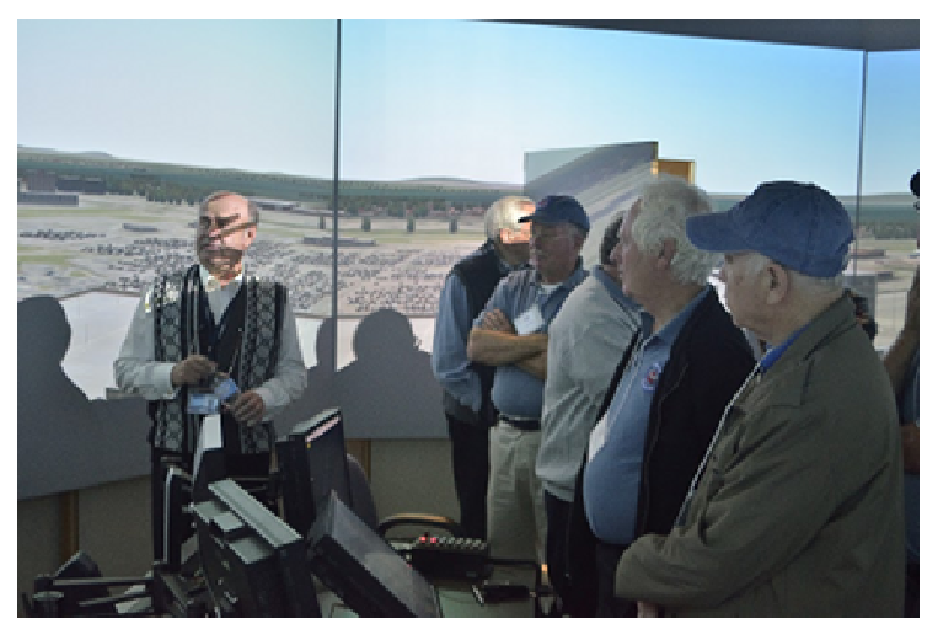
\includegraphics[scale=0.5]{yul_tca3.eps}
   %caption of the figure 
   \caption*{\small \em In the 360 degree tower simulator.}
   %label of the figure, which has to correspond to \ref{}:
   \label{fig:tca3}
\end{figure}

Our next stop was the Technical Operations Centre where staff monitor
all radar and computers. ACC has dual systems with one system picking
up automatically in case the other system fails. Communications has a
dual back-up digital and analogue system.  Communications to aircraft
are by conventional VHF with some interesting back ups such as
Controller Pilot Data Link Communications (CPDLC). The easiest way of
explaining this is Text Messaging Sat Com in which either the aircraft
can call the phone number of the ACC or the ACC can call the dedicated
number for the aircraft (\$6:00 a minute cost) and as a back up by HF
radio through a Flight Service Station.

\begin{figure}[htbp]
   \vspace{2em}
   \centering
   %name of the graphic, without the path AND in EPS format:
   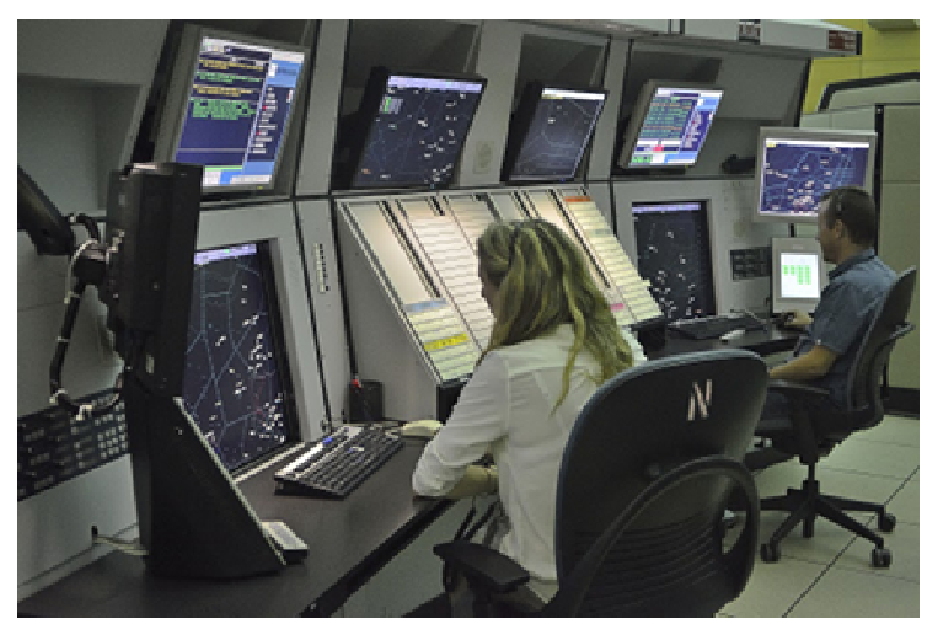
\includegraphics[scale=0.5]{yul_tca2.eps}
   %caption of the figure 
   \caption*{\small \em Air traffic controllers at work.}
   %label of the figure, which has to correspond to \ref{}:
   \label{fig:tca2}
\end{figure}

In the Operations Room, we could hear some controllers talking very
quietly. Radar displays offer a great deal of information to the
Controller, which also helps keep talking to a minimum. A sense of
humour prevailed at the work station for Northern Quebec up to
Iqaluit, where a Motel 6 logo was mounted over the work station.

In total we were on site for close to 2 1/2 hours which I found to be
a fantastic experience, seeing the ATC environment from the other
side.

\begin{figure}[htbp]
   \vspace{2em}
   \centering
   %name of the graphic, without the path AND in EPS format:
   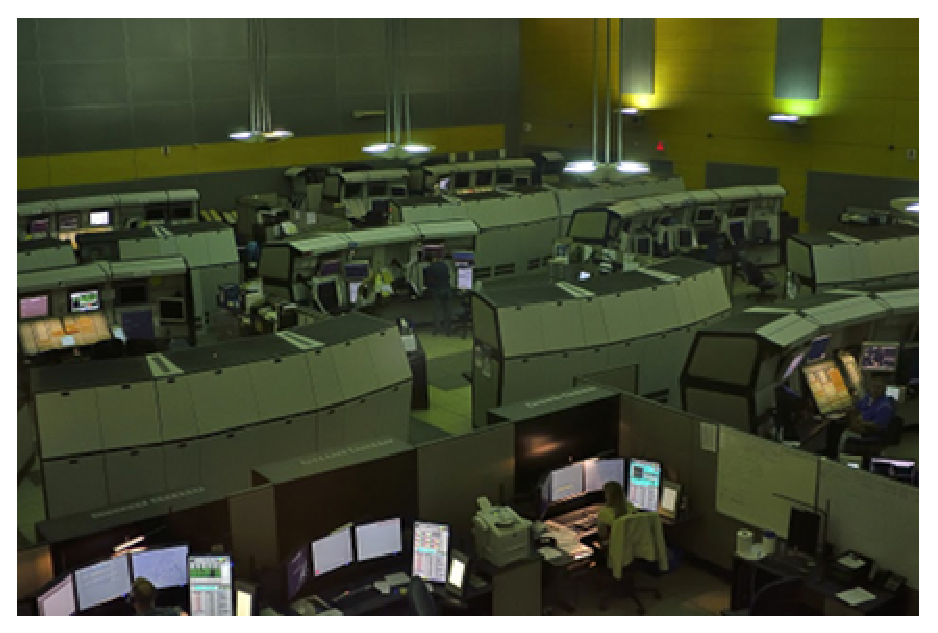
\includegraphics[scale=0.5]{yul_tca1.eps}
   %caption of the figure 
   \caption*{\small \em The Operations Room.}
   %label of the figure, which has to correspond to \ref{}:
   \label{fig:tca1}
\end{figure}

With kind assistance in the form of a recommendation from Mae, my YUL
expert, we broke off for lunch at Le D\'{e}jeuner Cosmopolitain which
handled our group in a very friendly efficient manner. I should note,
this is the spot where Air Canada retirees meet for their monthly
luncheon dates.

After lunch we proceeded to the Bombardier Production plant where we
were met by three very knowledgeable tour guides. They were Alex
Ritchie, Fernand Richer, and Cristian Racine who together gave a very
informed hour and half tour of the production line. The tour was
divided into two areas, assembly and finishing. At the beginning of
the assembly we saw where the fuselage and wings are mated and
proceeded on to where systems are tested such as hydraulic systems,
then to the finishing area where interiors are installed. It was
something to see how clean and bright this plant is and how the many
sub assemblies come together. The tail assembly built in China comes
to the production line and meets with part of the fuselage built in
Mexico, just in time for the assembly.

We ended our visit in the delivery room where customers pick up their
aircraft all ready to go, all yours for approximately \$30 million
dollars.

We enjoyed an excellent dinner at the Auberge Willow Inn prior to our
return to the CASM at the end of a very enjoyable 14 1/2 hour day
together.

\begin{footnotesize}
    \raggedleft PNSAC\\
\end{footnotesize}

%%% Local Variables: 
%%% mode: latex
%%% TeX-master: main_document.tex
%%% End: 
